Um sistema de pêndulo invertido consiste em uma haste suspensa verticalmente sobre um carro motorizado, como mostrado na Figura \ref{fig:diagrama-pendulo-invertido}. O objetivo do controle de atitude, que é referente ao controle de orientação angular, é manter a haste na posição vertical mesmo após o sistema sofrer alguma perturbação. Como o pêndulo invertido é um sistema instável, após sofrer esta perturbação a haste deverá cair a menos que uma ação de controle adequada seja exercida.

Neste exemplo, é considerado um problema bidimensional, em que o pêndulo se move apenas para a direita e para esquerda (i.e.\ no plano da página), mas não para frente e para trás (i.e\ no plano ortogonal a ela). Outra simplificação feita é a consideração de que o centro de gravidade da haste do pêndulo seja seu centro geométrico.

%\begin{figure}[!htb]
%    \centering
%    \caption{Diagrama do sistema de pêndulo invertido; (a) sistema de pêndulo invertido; (b) diagrama de corpo livre}
%    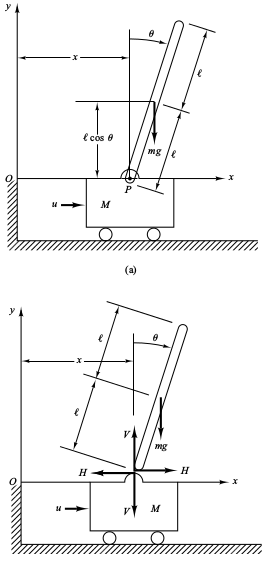
\includegraphics[width=0.55\textwidth]{./04-figuras/Ogata2010_inverted_pendulum_diagram_complete}
%    \fonte{\citeonline[p.~69]{Ogata2010}}
%    \label{fig:Ogata2010_inverted_pendulum_diagram_complete}
%\end{figure}
\begin{figure}[!htb]
    \centering
    \caption{Diagrama do sistema de pêndulo invertido}
    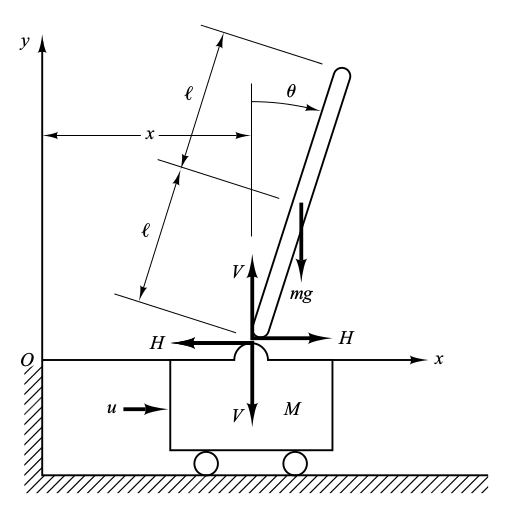
\includegraphics[width=0.6\textwidth]{./04-figuras/sistemas-nao-lineares/diagrama-pendulo-invertido}
    \fonte{Adaptado de \citeonline[p.~69]{Ogata2010}}
    \label{fig:diagrama-pendulo-invertido}
\end{figure}
%diagrama-pendulo-invertido

Além disso, o sistema mostrado na Figura \ref{fig:diagrama-pendulo-invertido}, assume que uma força $u$ seja aplicada ao carro, considerando $M$ como a massa do carro, $m$ a massa da haste, $g$ a força da gravidade, $x$ o deslocamento no eixo horizontal, $l$ a metade do comprimento da haste, $\theta$ o ângulo da haste com relação ao eixo vertical, $P$ o ponto de rotação do pêndulo sobre o carro, $H$ o movimento horizontal do centro de gravidade da haste do pêndulo e $V$ o movimento vertical do centro de gravidade da haste do pêndulo.

Com estes parâmetros, \citeonline[p.~69]{Ogata2010} mostra que o sistema descrito pode ser representado da seguinte maneira  no espaço de estados:
\begin{center}\label{eq:k1}
$\dot{x}=Ax+Bu$ \\
$y=Cx+Du$
\end{center}
em que:
%\begin{equation*}
%x=
%\left[ \begin{array}{@{}*{4}{c}@{}}
%     \theta & \dot{\theta} & x & \dot{x} \\
%\end{array} \right]^T
%\end{equation*}
%
%Além disto, o vetor $y$ de saída do sistema foi definido como:
\[
%	x =
%	\begin{bmatrix}
%	\theta & \dot{\theta} & x & \dot{x}
%	\end{bmatrix}^T\quad
	x =
		\begin{bmatrix}
		\theta \\ \dot{\theta} \\ x \\ \dot{x}
		\end{bmatrix}\quad
	y = 
	\begin{bmatrix}
			\theta \\
			x
	\end{bmatrix}
\]
\[
	A = 
	\begin{bmatrix}
		0 & 1 & 0 & 0 \\
		\frac{M+m}{Ml}g & 0 & 0 & 0 \\
		0 & 0 & 0 & 1 \\
		-\frac{m}{M}g & 0 & 0 & 0
	\end{bmatrix}\quad
	B = 
	\begin{bmatrix}
		0 \\
		-\frac{1}{Ml} \\
		0 \\
		\frac{1}{Ml}
	\end{bmatrix}
\]

\[
	C = 
		\begin{bmatrix}
			1 & 0 & 0 & 0 \\
			0 & 0 & 1 & 0
		\end{bmatrix}\quad
	D = 
		\begin{bmatrix}
			0 \\
			0
		\end{bmatrix}
\]

Como o sistema de pêndulo invertido não é o foco deste trabalho, sendo referenciado apenas como uma analogia para sistemas não-lineares instáveis, o desenvolvimento da modelagem matemática mostrado por \citeonline[p.~70]{Ogata2010} não foi explicitado.

Uma vez exibido um modelo de um sistema instável mais simples, pode-se melhor compreender a modelagem de um sistema mais complexo como é o de um quadrotor, assunto este que é abordado na próxima seção.
%Desta forma, se obtém a representação completa do sistema de pêndulo invertido no espaço de estados.
%Este sistema foi modelado por \citeonline[p.~69]{Ogata2010}
%\hl{Inserir diagrama de blocos do sistema}\\